\chapter{\uppercase{RESULTS AND EVALUATION}}
\label{Capitulo 6}

Purpose of this chapter is to present the evaluation's results of proposed  anomaly detection mechanism, to later show some of results obtained with it.
%El prop\'{o}sito de este cap\'{i}tulo es presentar los resultados de la evaluaci\'{o}n del mecanismo de detecci\'{o}n de anomal\'{i}as propuesto, para posteriormente mostrar algunos de los resultados obtenidos con el mismo.

\section{Performance evaluation}

This study will evaluate the effectiveness of anomaly detection techniques from following two perspectives:
\begin{itemize}
\item The ability of approach to distinguish between normal and anomalous data.
\item The efficiency of method according to time required to train model and time spent during detection process.
\end{itemize}
%En este estudio se evaluar\'{a} la efectividad de las t\'{e}cnicas de detecci\'{o}n de anomal\'{i}as desde las dos siguientes perspectivas:
%\begin{itemize}
%\item La capacidad del enfoque para distinguir entre datos normales y an\'{o}malos.
%\item La eficiencia del m\'{e}todo de acuerdo con el tiempo requerido para entrenar el modelo y el tiempo empleado durante el proceso de detecci\'{o}n.
%\end{itemize}

\subsection{Evaluation in detection performance's terms}

Before evaluating the mechanism proposed in this study, it is important to highlight what:
%Antes de evaluar el mecanismo propuesto en este estudio es importante destacar qu\'{e}:

\begin{itemize}
\item \textbf{Normal behavior model} was trained with 21000 samples, during 50 iterations, with 4500 samples that were used to validate model during training stage, and finally test set with which the final evaluation of this model was made is compose with 4500 samples.
%\item El \textbf{modelo de comportamiento normal} fue entrenado con 21000 muestras, durante 50 iteraciones, con 4500 muestras que se usaron para validar el modelo durante la etapa de entrenamiento, y por \'{u}ltimo el conjunto de prueba con el que se realiz\'{o} la evaluaci\'{o}n final de este modelo esta conformado por 4500 muestras.
\item On the other hand, \textbf{anomaly detection method} was trained with all dataset that were used in the development of normal behavior model generation, that is, with 30,000 samples.
%\item Por otra parte el \textbf{m\'{e}todo detector de anomal\'{i}as} fue entrenado con la totalidad de los datos que se usaron en el desarrollo de la generaci\'{o}n del modelo del comportamiento normal, es decir, con 30000 muestras.
\end{itemize}

To evaluate the anomaly detection mechanism proposed in this study, following criteria were used: detection rate and false positive rate. Detection rate is defined as the number of detected anomalies divided by total number of anomalies. False positive rate is defined as the number of "normal" series that are classified as anomalies divided by the total number of "normal" series. It is important to clarify that outliers' set, available in this research, was not used for training the proposed method; however, this set was used to validate its precision, therefore data set with which this mechanism is validated has 44204 data.
%Para evaluar el mecanismo de detecci\'{o}n de anomal\'{i}as propuesto en el estudio, se utiliz\'{o} los siguientes criterios: la tasa de detecci\'{o}n y la tasa de falsos positivos. La tasa de detección se define como el número de anomal\'{i}as detectadas dividido por el número total de anomal\'{i}as. La tasa de falsos positivos se define como el número de series ''normales'' que se clasifican como anomal\'{i}as divididos por el número total de series ''normales''. Es importante aclarar que el conjunto de valores at\'{i}picos, con el que se cuenta en esta investigaci\'{o}n, no fue usado para el entrenamiento del m\'{e}todo propuesto; sin embargo este conjunto s\'{i} se us\'{o} para validar su precisi\'{o}n, por lo tanto el conjunto de datos con el que se valida este mecanismo cuenta con 44204 datos.
 
\vspace{5mm} %5mm vertical space

Table \ref{table:matriz_resultado} presents confusion matrix obtained by the proposed mechanism, from which following statements can be obtained:
%En la Tabla \ref{table:matriz_resultado} se presenta la matriz de confusi\'{o}n obtenida por el mecanismo propuesto, de donde se pueden obtener las siguientes afirmaciones:

\begin{itemize}
\item Upper left entry in matrix shows that 111 anomalies out of 164 were correctly labeled, that is, that 67.68\% of anomaly samples were correctly recognized.
%\item La entrada superior izquierda de la matriz muestra que 111 anomal\'{i}as de 164 fueron correctamente etiquetas, es decir, que el 67.68\% de las muestras de anomal\'{i}as se reconocieron correctamente.
\item Bottom row shows that 43688 of 44040 data were correctly labeled as normal values, i.e. 99.20\%. Therefore false positive rate for normal class is $100−99.20\% = 0.80\%$.
%\item En la fila inferior se muestra que 43688 de 44040 datos fueron etiquetadas correctamente como valores normales, es decir, el 99.20\%. Por lo tanto la tasa de falsos positivos para la clase normal es $100-99.20\% = 0.80\%$.
\end{itemize}

\begin{table}[H]

\centering
\begin{center}
\begin{tabular}{ll|c|c|}
\cline{3-4}
                                                        &                                              & \multicolumn{2}{c|}{\textbf{Prediction}}                                                          \\ \cline{3-4} 
                                                        &                                              & \textbf{Anomaly}                         & \textbf{Normal Class}                         \\ \hline
\multicolumn{1}{|c|}{}                                  & \multicolumn{1}{c|}{\textbf{Anomaly}} & \cellcolor[HTML]{AADD99}111 & \cellcolor[HTML]{FFCE93}53 \\ \cline{2-4} 
\multicolumn{1}{|c|}{\multirow{-2}{*}{\textbf{Real}}} & \multicolumn{1}{c|}{\textbf{Normal Class}} & \cellcolor[HTML]{DF9F9F}352 & \cellcolor[HTML]{AADD99}43688 \\ \hline
\end{tabular}
\caption{Confusion matrix, for the anomaly detection mechanism (Own elaboration).}
\label{table:matriz_resultado}
\end{center}
\end{table}

These results are a great advance for conduction anomalies' detection with a semi-supervised approach, since without having samples of outliers in training, it is difficult to have a higher precision; considering also that one of the most important added values presented by this research work, is to be able to generate a personalized model for each agent's type, which is really outstanding, because related work that was reviewed (prior to carry out this investigation) does not have an exemplary that contemplates a semi-supervised approach, much less with models that are adjusted and personalized for each agent.
%Estos resultados son un gran avance para la detecci\'{o}n de anomal\'{i}as de conducci\'{o}n con un enfoque semi supervisado, ya que al no contar con muestras de valores at\'{i}picos en el entrenamiento es dif\'{i}cil tener una precisi\'{o}n m\'{a}s alta; considerando adem\'{a}s, que uno de los valores agregados m\'{a}s importantes que presenta este trabajo de investigaci\'{o}n, es el poder generar un modelo personalizado por cada tipo de agente, lo cual es realmente sobresaliente, debido a que el trabajo relacionado que se revis\'{o}, previamente a la elaboraci\'{o}n de esta investigaci\'{o}n, no cuenta con un ejemplar que contemple un enfoque semi-supervisado y mucho menos con modelos que se ajusten y personalicen para cada agente.

%\subsection{Evaluación en términos de tiempo de ejecución}

\section{Results}

Results of this study provide an essential contribution in the field of automation of early abnormal behaviors' detection in car driving; However, these present an overview of the behavior of the proposed model, so it is necessary to carry out a more specific analysis of said behavior with each type of anomaly presented in data set, as well as the analysis of those values that were detected wrongly as anomalies (false positives). The results of previously mentioned analyzes are presented below.
%Los resultados de este estudio proporcionan una contribuci\'{o}n esencial en el campo de la automatizaci\'{o}n de  detecci\'{o}n temprana de conductas an\'{o}malas en la conducci\'{o}n de autom\'{o}viles; sin embargo, \'{e}stos presentan una visi\'{o}n general del comportamiento del modelo propuesto, por lo cual es necesario realizar un an\'{a}lisis m\'{a}s espec\'{i}fico de dicho comportamiento con cada tipo de anomal\'{i}a presentada en el conjunto de datos, as\'{i} como tambi\'{e}n el an\'{a}lisis sobre aquellos valores que fueron detectados err\'{o}neamente como anomal\'{i}as (falsos positivos). A continuaci\'{o}n se presentan los resultados de los an\'{a}lisis previamente mencionados.

%Aunque los resultados tengan cifras alentadoras, no se conoce a cabalidad como se detectan las anomal\'{i}as, en que casos se detectan falsos positivos y falsos negativos; por lo que a continuaci\'{o}n se presenta algunos de los resultados obtenidos por cada tipo de anomal\'{i}a del conjunto de valores at\'{i}picos. 

\subsection{Anomalies' detection of zig zag type}

This anomaly corresponds to a common behavior for agents who drive under the influence of alcohol; it consists of driving that presents sudden zig zag movements, that is, constant changes of direction and at a relatively high speed. Below are some of results that were obtained with anomaly detection mechanism proposed in this research work.
%Esta anomal\'{i}a corresponde a un comportamiento com\'{u}n que suelen realizar agentes que conducen bajo los efectos del alcohol; consiste en una conducci\'{o}n que presenta movimientos en zig zag de forma brusca, es decir, cambios de direcci\'{o}n constante y a una velocidad relativamente alta. A continuaci\'{o}n se presenta algunos de los resultados que se obtuvo con el mecanismo de detecci\'{o}n de anomal\'{i}as propuesto con este trabajo de investigaci\'{o}n.

\begin{figure}[H]
        \centering
        
\fbox{\begin{varwidth}{\textwidth}
        \centering
        \begin{subfigure}[h]{0.45\textwidth} 
            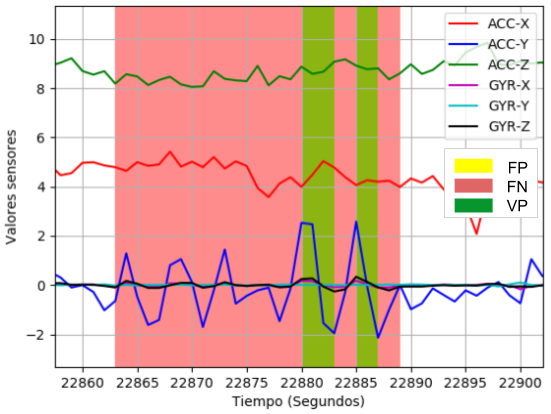
\includegraphics[width=\textwidth]{imagenes/Cap5/zig_zag1}
        \end{subfigure}       
        \begin{subfigure}[h]{0.45\textwidth} 
            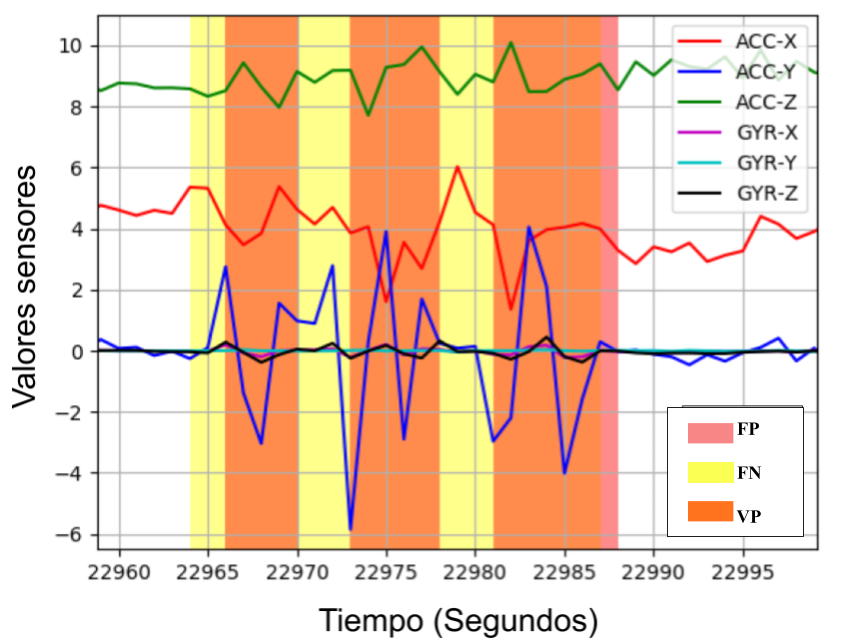
\includegraphics[width=\textwidth]{imagenes/Cap5/zig_zag2}
        \end{subfigure}
        \begin{subfigure}[h]{0.45\textwidth} 
            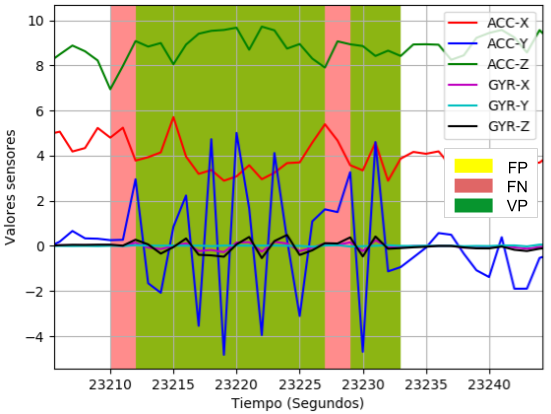
\includegraphics[width=\textwidth]{imagenes/Cap5/zig_zag3}
        \end{subfigure} 
        \end{varwidth}}
        \caption{Results of anomalies' detection of zig zag type (Own elaboration).}
		\label{fig:resultados_zigzag}
    \end{figure}
 
Before carrying out the results obtained's analysis, it should be clarified that those sections of following graphs that appear in red are the values that belong to anomalies' set that were not correctly detected (False negatives), the sections in yellow correspond to false positives and finally the green sections are true positives, that is, those values that were correctly detected as anomalies.   
%Antes de realizar el an\'{a}lisis de los resultados obtenidos se debe aclarar que aquellas secciones de las siguientes gr\'{a}ficas que se presentan en color rojo son los valores que pertenecen al conjunto de anomal\'{i}as que no fueron correctamente detectados (Falsos negativos), las secciones en amarillo corresponden a los falsos positivos y por \'{u}ltimo las secciones verdes son los verdaderos positivos, es decir, aquellos valores que fueron detectados correctamente como anomal\'{i}as.

\vspace{5mm} %5mm vertical space

As seen in Figure 6.1, upper left image presents a large number of false negatives, this is because the movements' oscillations in Zig Zag were not sudden enough, compared to others, on the other hand, image upper right presents a moderate number of false negatives and one false positive specimen, although result does not seem quite good really, it is good, since many of false negatives are among correctly detected values, which would lead to a correct alarm generation despite not detecting as an outlier all anomalous data, a similar example is presented in image below, although in this case no false positives are detected.
%Como se observa en la Gr\'{a}fica \ref{fig:resultados_zigzag}, la imagen superior izquierda presenta una gran cantidad de falsos negativos, esto se debe a que las oscilaciones de los movimientos en Zig Zag no fueron lo suficientemente bruscos, en comparaci\'{o}n a los dem\'{a}s, por otro lado la imagen superior derecha presenta una cantidad moderada de falsos negativos y un ejemplar de falso positivo, aunque el resultado no parezca del todo bueno realmente si lo es, ya que muchos de los falsos negativos se encuentran entre valores detectados correctamente, lo cual conllevaria a una correcta generaci\'{o}n de alarma de anomal\'{i}as a pesar de no detectar como valor at\'{i}pico la totalidad de los datos an\'{o}malos, en la imagen inferior se presenta un ejemplo similar, aunque en este caso no se detectan falsos positivos.

In order to formalize results for Zig Zag anomalies, in table 6.2 it can be seen that 69 anomalies out of 105 were correctly detected, that is, 65.71\%.
%Con el fin de formalizar los resultados para las anomal\'{i}as del tipo Zig Zag, en la tabla \ref{table:zigzag_resultado} se puede observar que 69 anomal\'{i}as de 105 fueron correctamente detectadas, es decir el 65.71\%. 

\begin{table}[H]
\centering
\begin{center}
\begin{tabular}{|c|c|c|}
\hline
\multicolumn{3}{|l|}{\textbf{Zig Zag turns}} \\ \hline
\textbf{TP}   & \textbf{FN}   & \textbf{Total}  \\ \hline
\cellcolor[HTML]{AADD99}69  & \cellcolor[HTML]{DF9F9F}36  & 105             \\ \hline
\end{tabular}
\caption{Results of anomalies Zig Zag type (Own elaboration).}
\label{table:zigzag_resultado}
\end{center}
\end{table}

\subsection{Anomalies' detection for turns at high speed}

This type of anomalies are usually common in agents who drive under the influence of alcohol, drugs or with an altered emotional state, these data are considered anomalies since turns are normally made by lowering of vehicle's speed, and when performing these types of acts an agent is prone to being the cause of a traffic accident.
%Este tipo de anomal\'{i}as suelen ser comunes en agentes que conducen bajo los efectos del alcohol, drogas o con un estado emocional alterado, dichos datos se consideran anomal\'{i}as ya que los giros normalmente se realizan bajando la velocidad del veh\'{i}culo, y al realizar este tipo de actos un agente es propenso a ser el causante de un accidente de tr\'{a}nsito.

\vspace{5mm} %5mm vertical space

Figure \ref{fig:resultados_giros} shows results obtained for high speed turns anomalies, the three images present very similar results, all have a section in initial part that is presented as false negative, that is, they have a number of data that are not correctly detected, later they have a block of true positives, and finally, two of three images have a false positive specimen after the anomaly. Although these types of anomalies are not completely detected, they all have a section that is detected as an anomaly, which is enough to generate an alarm in a timely manner.
%La Figura \ref{fig:resultados_giros} muestra los resultados obtenidos para las anomal\'{i}as del tipo giros a alta velocidad, las tres imagenes presentan resultados muy similares, todas tienen una secci\'{o}n en la parte inicial que se presenta como falso negativo, es decir tienen una proporci\'{o}n de datos que no son detectadas correctamente, posteriormente cuentan con un bloque de verdaderos positivos, y por \'{u}ltimo, dos de las tres imagenes cuentan con un ejemplar de falso positivo posterior a la anomal\'{i}a. A pesar de que este tipo de anomal\'{i}as no son detectadas completamente, todas presentan una secci\'{o}n que s\'{i} es detectado como anomal\'{i}a, lo cual es suficiente para generar una alarma oportunamente.

\begin{figure}[H]
        \centering
        
\fbox{\begin{varwidth}{\textwidth}

        \centering
        \begin{subfigure}[h]{0.45\textwidth} 
            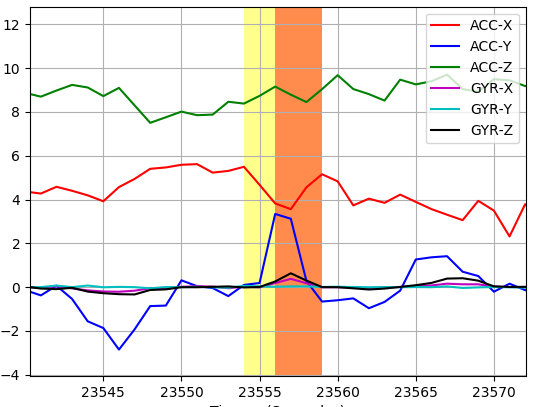
\includegraphics[width=\textwidth]{imagenes/Cap5/giro1}
        \end{subfigure}       
        \begin{subfigure}[h]{0.45\textwidth} 
            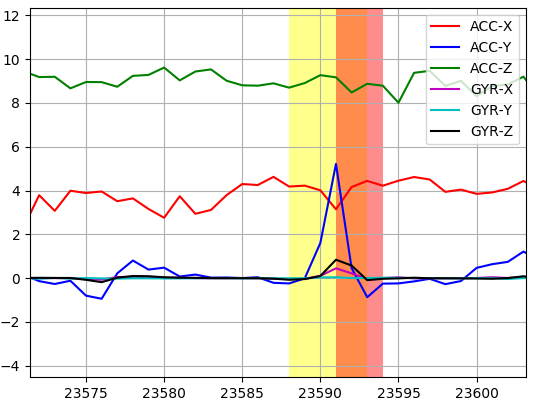
\includegraphics[width=\textwidth]{imagenes/Cap5/giro2}
        \end{subfigure}
        \begin{subfigure}[h]{0.45\textwidth} 
            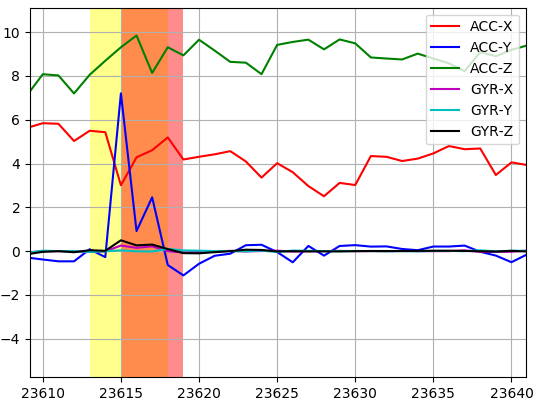
\includegraphics[width=\textwidth]{imagenes/Cap5/giro3}
        \end{subfigure} 
        \end{varwidth}}
        \caption{Results of anomalies' detection of the high speed turns type (Own elaboration)}
		\label{fig:resultados_giros}
    \end{figure}

Table \ref{table:giros_resultado} presents the general results obtained for high speed turns anomalies, where of 35 anomalies, 23 were correctly detected, that is, 65.71\%.
%En el Cuadro \ref{table:giros_resultado} se presenta los resultados generales obtenidos para las anomal\'{i}as del tipo Giros a alta velocidad, donde de 35 anomal\'{i}as 23 fueron correctamente detectadas , es decir, el 65.71\%.

\begin{table}[H]
\centering
\begin{center}
\begin{tabular}{|c|c|c|}
\hline
\multicolumn{3}{|l|}{\textbf{High speed turns}} \\ \hline
\textbf{TP}   & \textbf{FN}   & \textbf{Total}  \\ \hline
\cellcolor[HTML]{AADD99}23  & \cellcolor[HTML]{DF9F9F}12  & 35             \\ \hline
\end{tabular}
\caption{Results anomalies' detection of the type High speed turns (Own elaboration).}
\label{table:giros_resultado}
\end{center}
\end{table}

\subsection{Anomalies' detection of the type dry brakes}

This type of anomaly is usually one of the most common outliers that exist, since they not only occur under the influence of alcohol, drugs or mechanical failures, but also occur in contexts of driver distraction due to the cell phone's use or other distraction's type, when a pedestrian or pet appears suddenly in the lane that the agent drives, among other cases.
%Este tipo de anomal\'{i}a suele ser uno de los valores at\'{i}picos m\'{a}s comunes que existen, ya que no s\'{o}lo se presentan bajo los efectos del alcohol, drogas o fallas mec\'{a}nicas, sino que tambi\'{e}n se presentan en contextos de distracci\'{o}n del conductor ya sea por el uso del celular u otro tipo de distracci\'{o}n, ante la aparici\'{o}n de un peat\'{o}n o mascota que se presenta de manera repentina en la carril que conduce el agente, entre otros casos.

\vspace{5mm} %5mm vertical space

Detection's results of this type of anomaly are presented in Figure \ref{fig:resultados_frenos}, where, as in previous case, this type of anomaly presents a section of false negatives, later a group of anomalies correctly detected and finally false positives; with which it is enough to generate alerts in a timely manner and thus be able to avoid any possible traffic accident.
%Los resultados de la detecci\'{o}n de este tipo de anomal\'{i}a se presentan en la Figura \ref{fig:resultados_frenos}, donde al igual que el caso anterior este tipo de anomal\'{i}a presenta una secci\'{o}n de falsos negativos, posteriormente un grupo de anomal\'{i}as correctamente detectadas y finalmente falsos positivos; con lo cual es suficiente para generar alertas de manera oportuna y de esa manera poder evitar en lo posible alg\'{u}n accidente de tr\'{a}nsito.

\begin{figure}[H]
        \centering
\fbox{\begin{varwidth}{\textwidth}
        \centering
        \begin{subfigure}[h]{0.45\textwidth} 
            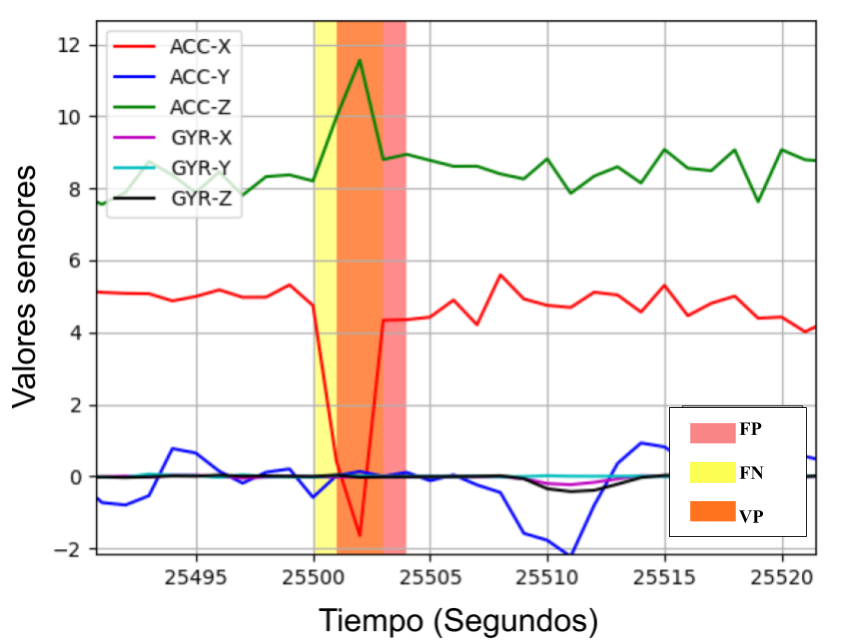
\includegraphics[width=\textwidth]{imagenes/Cap5/freno1}
        \end{subfigure}       
        \begin{subfigure}[h]{0.45\textwidth} 
            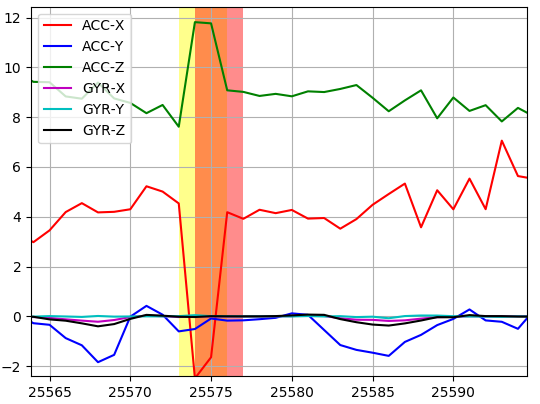
\includegraphics[width=\textwidth]{imagenes/Cap5/freno2}
        \end{subfigure}
        \begin{subfigure}[h]{0.45\textwidth} 
            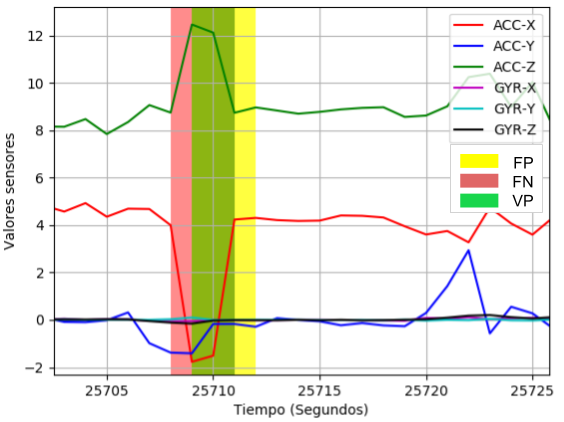
\includegraphics[width=\textwidth]{imagenes/Cap5/freno3}
        \end{subfigure} 
        \end{varwidth}}
        \caption{Results of anomalies' detection of type dry brakes (Own elaboration).}
		\label{fig:resultados_frenos}
    \end{figure}

Below in Table 6.4 it can be seen that 19 anomalies out of 24 were correctly detected (79.17\%), thus being this anomaly's type that has the highest detection percentage.
%A continuaci\'{o}n en el Cuadro \ref{table:frenos_resultado} se puede ver que 19 anomal\'{i}as de 24 fueron correctamente detectadas (79.17\%), siendo as\'{i} el tipo de anomal\'{i}a que tiene el porcentaje de detecci\'{o}n m\'{a}s elevado.

\begin{table}[H]
\centering
\begin{center}
\begin{tabular}{|c|c|c|}
\hline
\multicolumn{3}{|l|}{\textbf{Dry brakes}} \\ \hline
\textbf{TP}   & \textbf{FN}   & \textbf{Total}  \\ \hline
\cellcolor[HTML]{AADD99}19  & \cellcolor[HTML]{DF9F9F}5  & 24             \\ \hline
\end{tabular}
\caption{Results of anomalies' detection of the type dry brakes (Own elaboration).}
\label{table:frenos_resultado}
\end{center}
\end{table}

\subsection{Detection of false positives}

Just as a large number of anomalies were detected using this mechanism, a considerable proportion of false positives were also detected, that is, normal values that were erroneously detected as outliers.
%As\'{i} como se detect\'{o} una gran cantidad de anomal\'{i}as mediante este mecanismo, tambi\'{e}n se detect\'{o} una proporci\'{o}n considerable de falsos positivos, es decir, valores normales que fueron detectados err\'{o}neamente como valores at\'{i}picos.

\vspace{5mm} %5mm vertical space

In the same way that it is important to know how this method detects anomalies, it is also important to know in which cases the proposed model fails; Figure \ref{fig:resultados_falsos_positivos} shows some cases where the model fails, that is, this figure presents some false positives' examples. Figure \ref{fig:resultados_falsos_positivos} clearly illustrates that these false positives are generally presented in isolation, that is, one or two values erroneously detected as anomalies continuously, which is a different behavior from true outliers, since these present a detection minimally three outliers continuously.
%De la misma forma que es importante conocer como este m\'{e}todo detecta anomal\'{i}as, tambi\'{e}n es importante saber en que casos el modelo propuesto falla; en la Figura \ref{fig:resultados_falsos_positivos} se presenta algunos casos donde el modelo falla, es decir, esta figura presenta algunos ejemplos de falsos positivos. La figura \ref{fig:resultados_falsos_positivos} ilustra claramente que estos falsos positivos se presentan generalmente de forma aislada, es decir, uno o dos valores detectados err\'{o}neamente como anomal\'{i}as de forma continua, lo cual es un comportamiento diferente al de los verdaderos valores at\'{i}picos, ya que estos presentan una detecci\'{o}n de tres valores at\'{i}picos de forma continua m\'{i}nimamente.

\begin{figure}[H]
        \centering
\fbox{\begin{varwidth}{\textwidth}
        \centering
        \begin{subfigure}[h]{0.45\textwidth} 
            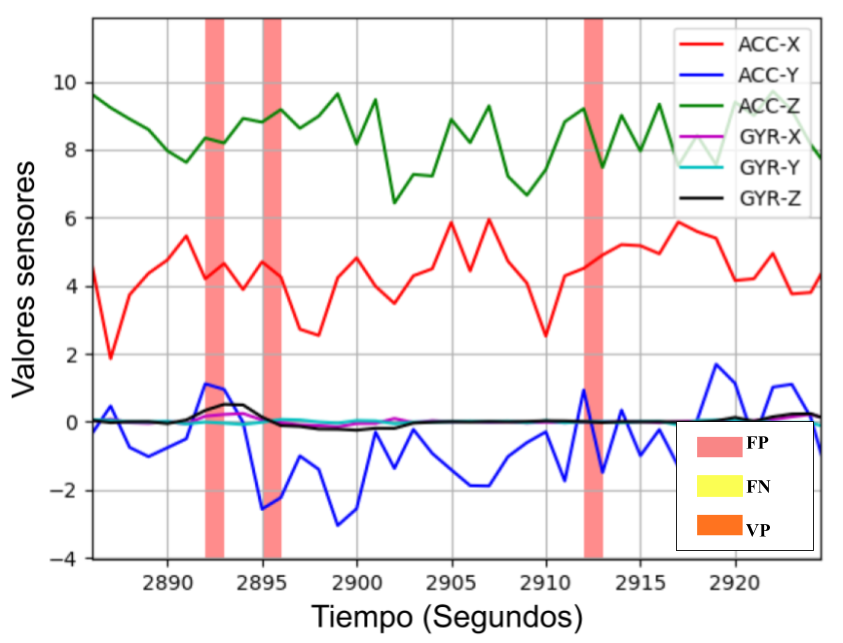
\includegraphics[width=\textwidth]{imagenes/Cap5/fp1}
        \end{subfigure}       
        \begin{subfigure}[h]{0.45\textwidth} 
            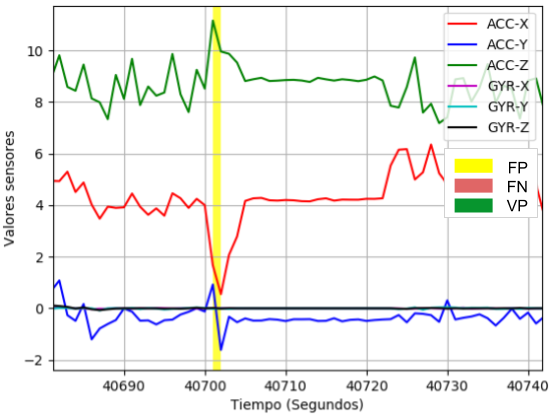
\includegraphics[width=\textwidth]{imagenes/Cap5/fp2}
        \end{subfigure}
        \begin{subfigure}[h]{0.45\textwidth} 
            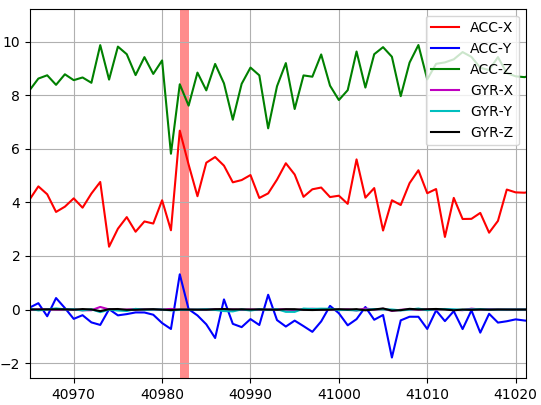
\includegraphics[width=\textwidth]{imagenes/Cap5/fp3}
        \end{subfigure} 
        \end{varwidth}}
        \caption{Results of false positives' detection (Own elaboration).}
		\label{fig:resultados_falsos_positivos}
    \end{figure}

%\section{Resumen}

%Este cap\'{i}tulo detall\'{o} el tipo de evaluaci\'{o}n al que se someti\'{o} el mecanismo propuesto en el trabajo de investigaci\'{o}n, para finalmente presentar los resultados que se obtuvieron por cada tipo de anomal\'{i}a.
 
 